% Aidan Hunt
% ME 498 K
% Spring 2023
% Homework 5

\documentclass{homework}
\usepackage[utf8]{inputenc}
\usepackage{amsmath}
\usepackage{amssymb}
\usepackage{braket}
\usepackage{bm}
\usepackage{caption}

% Packages for presenting code
\usepackage{listings}
\usepackage{pythonhighlight}
\usepackage{graphicx}

\lstdefinestyle{BashOutputStyle}{
  basicstyle=\footnotesize\ttfamily,
  numbers=none,
  frame=tblr,
  columns=fullflexible,
  backgroundcolor=\color{blue!10},
  linewidth=0.9\linewidth,
  xleftmargin=0.1\linewidth
}

% Packages for presenting output
\usepackage{hyperref}
\hypersetup{
    colorlinks=true,
    linkcolor=blue,
    filecolor=magenta,      
    urlcolor=blue,
    }

\raggedbottom

%use \question*{Title} to title a question

% make short commands for subproblem listing
\newcommand{\substart}{\begin{enumerate}[label={(\alph*)}]}
\newcommand{\subend}{\end{enumerate}}

%Instructor info
\newcommand{\hwname}{Aidan Hunt}
\newcommand{\hwemail}{ahunt94@uw.edu}

%Assignment type
\newcommand{\hwtype}{Homework}

%Class info
\newcommand{\hwclass}{ME 498 K}
\newcommand{\hwterm}{Spring 2023}

%Assignment specifics
\newcommand{\hwnum}{6}
\newcommand{\hwduedate}{May 19th, 2023 and May 26, 2023}

% \newcommand{\uu}	    {{\mathrm{\textbf{u}}}}

\begin{document}
\maketitle

In this homework, you will practice defining Python classes and using instances of those classes to process data. You will also practice using the \texttt{os} and \texttt{glob} modules to process groups of similarly named and formatted files. Post questions about this assignment to the class discussion board for the fastest response. 

You will submit this homework in two stages:
\begin{itemize}
    \itemsep0em 
    \item[] \underline{\textbf{May 19th}:} Pseudocode outline due. Submit your outline to GradeScope as a single \texttt{.py} file. \textbf{You cannot use late days for your pseudocode outline.}
    \item[] \underline{\textbf{May 26th}:} Full assignment code due. Submit your code to GradeScope as a single \texttt{.py} file. You may use late days.
\end{itemize}


\subsubsection*{Background}

Load cells are sensors that use strain gauges to measure forces and/or torques in a system. In this homework, you will work with data from two ATI 6-axis load cells: one model \href{https://www.ati-ia.com/products/ft/ft_models.aspx?id=Mini45+IP65%2FIP68}{Mini45-IP65} and one model \href{https://www.ati-ia.com/products/ft/ft_models.aspx?id=Mini40+IP65%2fIP68}{Mini40-IP68}. These load cells measure 3 components of force ($F_X$, $F_Y$, $F_Z$) and 3 components of moment/torque ($M_X$, $M_Y$, $M_Z$). The two load cells are integrated into a laboratory scale cross-flow turbine test-rig for use in a recirculating water flume. Together, these load cells measure the net forces and torques on the turbine during operation, which helps us understand the hydrodynamics of these systems. If you'd like to know more about the physical system, you can read the methods section of \href{https://pubs.aip.org/aip/jrse/article/12/5/054501/1060548/Effect-of-aspect-ratio-on-cross-flow-turbine}{this paper we published in 2020}.

Using this system, an experiment was conducted in which the turbine performance was characterized at 18 different rotation rates. At each rotation rate, data was collected from all sensors in the system for 30 seconds at 1000 Hz and saved as a .csv file with the prefix "modelData". Each modelData file contains a $24\!\times\!30000$ matrix, where the rows correspond to particular sensors, and the columns correspond to samples in time. Your task is to process the raw data and produce a $6\times18$ aggregate data matrix of the \textbf{net, time-average} loads on the turbine as a function of rotation rate. The 6 rows of this data matrix will correspond to the six components of force/torque that the load cells measure: $F_X$, $F_Y$, $F_Z$, $M_X$, $M_Y$, and $M_Z$. The 18 columns correspond to \textbf{net} (i.e., the sum of both load cells) \textbf{time-average} loads at each of rotation rate.

\begin{figure}[h]
    \centering
    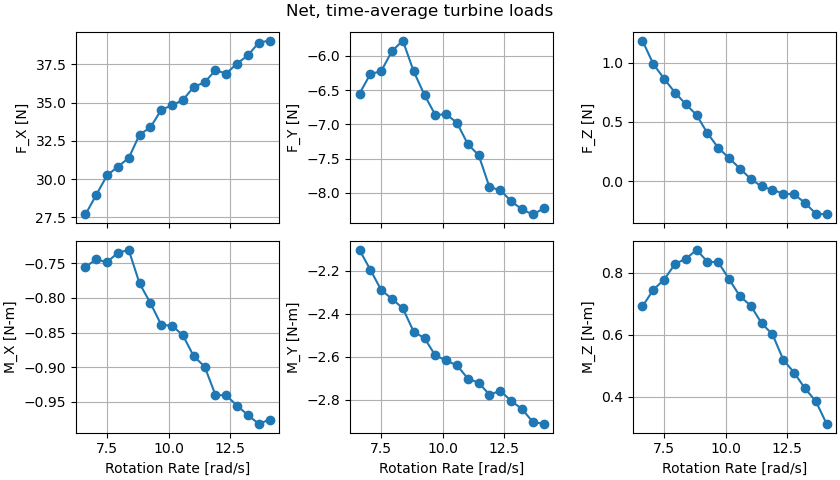
\includegraphics[width=0.75\textwidth]{exampleOutput.png}
\end{figure}

\newpage
\subsubsection*{Data conversion procedure}
% Show example output
For this assignment, only the following rows of each modelData file are relevant: 
\begin{itemize}
    \itemsep0em 
    \item[] Rows 1-6: Strain gauge readings from the upper Mini45-IP65 load cell, in Volts.
    \item[] Rows 7-12: Strain gauge readings from the lower Mini40-IP68 load cell, in Volts.
    \item[] Row 21: The turbine's angular velocity, in rad/s (this is constant for a given modelData file).
\end{itemize}

You may use the angular velocity as directly extracted from the data file, but we must convert the load cell readings to force in N and torques in N-m to interpret their physical meaning. This is accomplished via a multi-step post-processing procedure. For a $6\!\times\!N$ matrix of data from a \textbf{single} load cell:

\begin{minipage}{.4\linewidth}
    \begin{enumerate}
        \itemsep0em 
        \item \textbf{Subtract the tare from the measurements}. The tare reading is a $6\!\times\!1$ column vector that represents the output each strain gauge at zero load. This step is similar to zeroing a scale before weighing an item.
        \item \textbf{Apply the calibration matrix}. The $6\!\times\!6$ calibration matrix maps the contribution of each strain gauge to each component of force/torque. This should be applied as a matrix multiplication.
        \item \textbf{Apply the rotation matrix}. The $2\!\times\!2$ rotation matrix aligns the load cell readings in the $X$ and $Y$ directions (which are measured in a coordinate frame local to the load cell) with the global coordinate system based on the turbine. As for the previous step, this should be implemented as a matrix multiplication.
        \item \textbf{Flip readings of upper load cell}. The upper load cell in the system is mounted upside down. To account for this, the signs of the $F_Y$, $F_Z$, $M_Y$, and $M_Z$ readings \textbf{for the upper cell only} should be flipped.
    \end{enumerate}
\end{minipage}
\hfill
\begin{minipage}{.55\linewidth}
    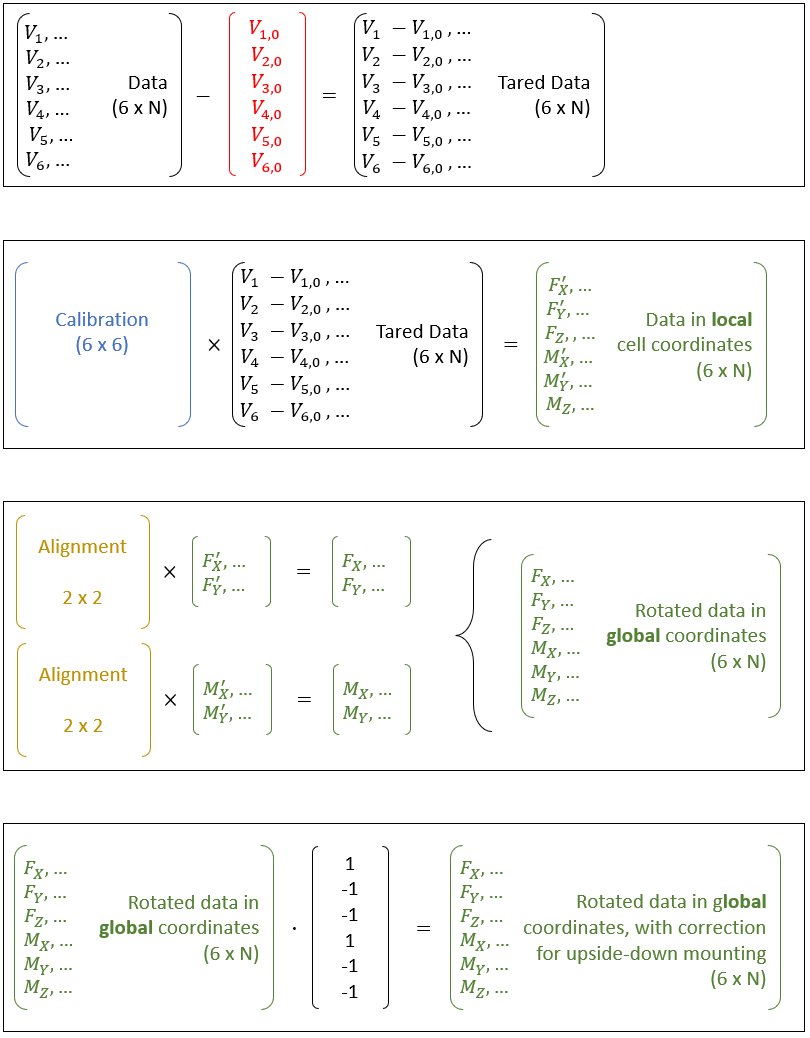
\includegraphics[width=\linewidth]{dataConversion.PNG}
\end{minipage}

Using this procedure, we can convert a $6\!\times\!30000$ matrix of strain gauge readings from a single load cell to $6\!\times\!30000$ matrix of forces and torques measured by that load cell. Then, for a given rotation rate, the net forces and torques on the turbine are obtained simply by summing the readings from the upper and lower load cells. Finally, the average net forces and torques at that rotation rate can be obtained by simply averaging along the appropriate dimension of the net data matrix.

The post-processing procedure outlined in steps 1-4 above is identical for each individual load cell, but depends on the \textit{state} of each individual load cell: for example, the load cell's tare, calibration, alignment (rotation matrix), and orientation (mounted in the upper or lower orientation). Because we would like to work data from \textit{individual sensors} that are both the same \textit{kind of object}...this is a great application for object-oriented programming!

\newpage
\subsubsection*{Defining the \texttt{LoadCell} class}

To process each load cell's data, you should define a \texttt{LoadCell} class that you can use to represent the physical load cells in the programming space. Your \texttt{LoadCell} class should have the following \textbf{attributes}:

\begin{tabular}{p{0.45\linewidth} | p{0.6\linewidth}} 
    \hline
    \texttt{LoadCell.model} & The model name of the load cell, as a string (e.g., \texttt{'Mini45-IP65'}). \\ \hline
    \texttt{LoadCell.dataIndex} & The indices of the rows in each modelData file that correspond to this load cell, as a list.  \\ \hline
    \texttt{LoadCell.orientation} & The mounting orientation of the load cell, as a string (e.g., \texttt{'upper'} or \texttt{'lower'}). \\ \hline
    \texttt{LoadCell.tare} & The tare reading for the load cell, as a NumPy array. \\ \hline
    \texttt{LoadCell.calMat} & The calibration matrix for the load cell, as a NumPy array. \\ \hline
    \texttt{LoadCell.rotMat} & The rotation matrix for the load cell, as a NumPy array. \\ \hline

\end{tabular}

Your \texttt{LoadCell} class should have the following \textbf{methods}:

\begin{tabular}{p{0.45\linewidth} | p{0.6\linewidth}} 
    \hline
    \texttt{LoadCell(model, dataIndex, orientation)} & Constructs a load cell object with the given model, data indices, and orientation. The \texttt{tare}, \texttt{calMat}, and \texttt{rotMat} attributes should be initialized to \texttt{None}. \\ \hline
    \texttt{LoadCell.postProcess(dataIn)} & Post processes a $6\!\times\!N$ NumPy array of strain gauge data from the load cell using Steps 1-4 of the procedure outlined in the previous section. The final $6\!\times\!N$ NumPy array of forces and torques is returned. \\ \hline
    \texttt{LoadCell.applyTare(dataIn)} & Given a $6\!\times\!N$ NumPy array of strain gauge data, subtracts the load cell's tare from the rows of the matrix and returns the result. \\ \hline
    \texttt{LoadCell.applyCalibration(dataIn)} & Given a $6\!\times\!N$ NumPy array of force/torque data, applies the load cell's calibration matrix to the data and returns the result. \\ \hline
    \texttt{LoadCell.applyRotation(dataIn)} & Given a $2\!\times\!N$ NumPy array of force/torque data, applies the load cell's rotation matrix to the data and returns the result. \\ \hline
    \texttt{LoadCell.flipSigns(dataIn)} & Given a $6\!\times\!N$ NumPy array of force/torque data, flips the signs of the values in the rows corresponding to $F_Y$, $F_Z$, $M_Y$, and $M_Z$ if the load cell is mounted in the upper orientation and returns the result. Otherwise, the original array is returned unaltered. \\ \hline
    \texttt{LoadCell.setTare(tareFile)} & Given the path to a .txt file (as a string) that contains this load cell's tare as a $6\!\times\!1$ column vector, sets the load cell's \texttt{tare} attribute to this vector. If the vector from the file is not a $6\!\times\!1$ column vector, a \texttt{ValueError} is raised and the \texttt{tare} attribute is not changed.  \\ \hline
    \texttt{LoadCell.setCalibration(calFile)} & Given the path to a .txt file (as a string) that contains this load cell's calibration matrix as a $6\!\times\!6$ matrix, sets the load cell's \texttt{calMat} attribute to this matrix (as a NumPy array). If the matrix from the file is not a $6\!\times\!6$ matrix, a \texttt{ValueError} is raised and the \texttt{calMat} attribute is not changed. \\ \hline
    \texttt{LoadCell.setRotation(rotFile)} & Given the path to a .txt file (as a string) that contains this load cell's rotation matrix as a $2\!\times\!2$ matrix, sets the load cell's \texttt{rotMat} attribute to this matrix (as a NumPy array). If the matrix from the file is not a $2\!\times\!2$ matrix, a \texttt{ValueError} is raised and the \texttt{rotMat} attribute is not changed. \\ \hline
\end{tabular}

You may assume that the user always provides inputs of the expected type, and that the files provided to the \texttt{.setTare}, \texttt{.setCalibration}, and \texttt{.setRotation} methods contain data that can be converted to NumPy arrays via \texttt{numpy.loadtxt}.

\newpage
\subsubsection*{Batch Processing the Data}

After defining the \texttt{LoadCell} class, you should create two instances of this class to represent the two load cells in the experimental system, and use these instances to batch process the data. Some guidelines:

\begin{itemize}
    \itemsep0em 
    \item In your batch processing routine, you should only load each modelData file \textbf{once}.
    \item To process each load cell's data, use the \texttt{.postProcess()} method of the corresponding object.
    \item You should use the \texttt{os} and \texttt{glob} modules to build paths to files of interest. To make grading easier for me, place the \texttt{Load Cell Data}, \texttt{Mini45-IP65 config}, and \texttt{Mini40-IP68 config} folders in the same directory as your script, and use relative paths.
    \item You should consider preallocating arrays in which to store any aggregated results.
    \item You should consider storing your \texttt{LoadCell} objects in a list (this will allow you to use your load cell objects in for loops).
    \item You should use the \texttt{.dataIndex} attribute of the \texttt{LoadCell} objects to help you identify the data that corresponds to each load cell.
\end{itemize}

\subsubsection*{Grading Criteria}

For this assignment, you will be graded based on both 1) your pseudocode outline and 2) your final assignment code.

Your pseudocode outline serves as a check-in to show me that you have started the assignment and spent a bit of time developing a plan for your program. To receive full credit, your pseudocode outline should demonstrate to me that you have identified the main components of the problem from the homework specification, and broken down these main components into sub-problems. Additionally, your pseudocode outline should include an outline of the \texttt{LoadCell} class, including its attributes and methods. You will not be graded on whether your outline is "right" or "wrong", but you will receive feedback from me to help guide your final assignment submission. See Lecture 12 for a good example of a pseudocode outline.

In terms of output, your final code will be graded on 1) whether it correctly implements the \texttt{LoadCell} class as requested, 2) whether the \texttt{LoadCell} objects are correctly used to post-process the data, 3) whether the \texttt{os} and \texttt{glob} modules are used correctly for identifying files for setting up the \texttt{LoadCell} objects and batch-processing, and 4) whether the requested aggregate data matrix is correctly produced. You may use the code posted on the class website to generate a figure to help check your results against the target output, but you will not be graded on this plot.

In terms of style, your final code should be well-structured and well-documented as always, and follow the Style Guide. Grading will be weighted more toward output, but you should still be on the lookout for any major redundancy and define functions to factor out repeated tasks. \textbf{Every} function (including methods belonging to the \texttt{LoadCell} class) must have a docstring that describes its parameters, returns, and any other behavior. The docstrings of \texttt{LoadCell} methods should describe how they alter the object attributes, if applicable. Remember, how your functions and methods respond to both valid and invalid user input cases is important behavior that should be documented.

You should be able to accomplish the tasks in this assignment with the object-oriented programming skills you have learned in class, the \texttt{os} and \texttt{glob} packages, and basic NumPy operations. If you need help with any aspect of this assignment, please post on the discussion board. Additionally, if you have any questions about general style requirements or the specific style requirements for this assignment, post them to the discussion board.

\end{document}

